\chapter{Charakterystyka EPUB}

\section{Omówienie}

EPUB jest standardem formatu dystrybucji cyfrowych publikacji i dokumentów opartych na standardach technologii webowej. EPUB definiuje
formę reprezentacji, organizacji struktury oraz kodowania określonej zawartości webowej, na co składają się XHTML, CSS, SVG, obrazy i
inne zasoby sprowadzone do formy pojedyńczego pliku. EPUB daje wydawcom możliwość stworzenia cyfrowej publikacji a następnie dystrybuowania
go, a odbiorcy łatwy dostęp do pliku niezależnie od urządzenia jakim operuje. Jako następca OEB (Open eBook Publication Structure),
zaprezentowanego w 1999 roku, EPUB 2 został ustandaryzowany w roku 2007 a aktualną jego wersją jest EPUB 3.1 (styczeń 2017). Dzisiaj jest
on standardem wykorzystywanym na szeroką skale przez wszystkich wydawców. Obok MOBI oraz PDF dominuje rynek, dzięki jego popularności
wsród wydawców oraz wsparciu urządzeń. W przeciwieństwie do MOBI które zostało spopularyzowane przez Amazon, właściciela sklepu amazon.com,
giganta dystybucji książek elektronicznych oraz producenta czytników elentronicznych marki Kindle, EPUB jest
standardem uniwersalnym, nieograniczonym do jednej platformy. EPUB zarówna jak i MOBI charakteryzuje się tym, że jego zawartość nie jest
statyczna, co oznacza, że ilość która jest wyświetlana dopasowana jest do wielkośći ekranu urządzenia dzięki czemu jest ona bardziej
przyjazna dla odbiorcy (PDF natomiast jest już podzielony na strony których nie da się podzielić). To co najbardziej różni EPUB od MOBI,
to wsparcie EPUB dla multimediów (od wersji 3.0) oraz CSS, który stulizuje cały dokument. Dzięki temu jest znacznie bardziej
elastyczny i nowoczesny. Popularną praktyką wśród dystrybutorów książek elektronicznych, jest dostarczanie ksiązki klientowi który ją
zakupił we wszystkich trzech wcześniej wymienionych formatach. EPUB jako standard jest szeroko udokumentowany dzięki International Digital
Publishing Forum\footnote{Adres url: \href{idpf.org}{idpf.org}}, grupie która nadrozuje rozwój formatu. W następnej sekcji zostanie
szczegółowo opisana struktura formatu EPUB.

\section{Specyfikacja}

Poniższa specyfikacja jest podzbiorem najważniejszych informacji wyselekcjonowanych ze specyfikacji EPUB 3.1 z dnia 5 stycznia 2017 roku
dostępnej na stronie International Digital Publishing Forum\footnote{Adres url najnowsej wersji specyfikacji: \href{http://www.idpf.org/epub3/latest}{http://www.idpf.org/epub3/latest}}.
Przedstawiono tutaj najbardziej istotne elementy formatu EPUB w celu zrozumienia problemu jakiego dotyczy projekt EPUBKit.

\subsection*{EPUB Open Container Format}

\begin{figure}[ht!]
  \centering
  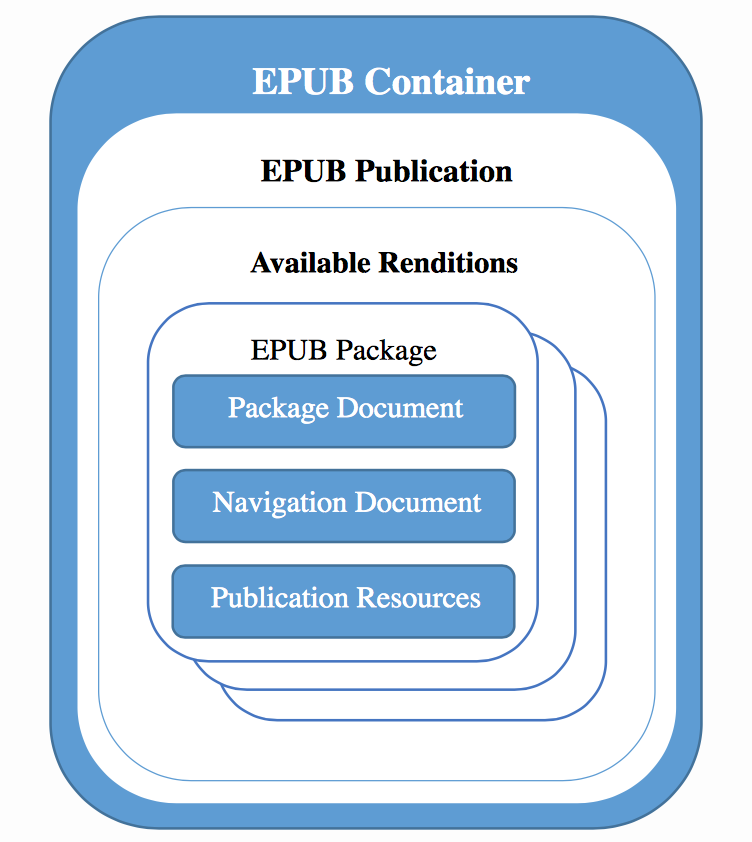
\includegraphics[width=.4\linewidth]{images/chapter-3-image-1-structure.png}
  \caption{Wizualna reprezentacja struktury formatu EPUB.\footnotemark}
  \label{chapter-3-image-1-structure}
\end{figure}
\footnotetext{Źródło: EPUB 3, Recommended Specification 5 January 2017, rozdział 2.2. Road Map.}

Format EPUB definiuje jego najwyższy abstrakcyjny model jakim jest EPUB Publication. Model ten składa się z interpretacji jego zawartości.
Interpretacja która jest przedstawiona za pomocą EPUB Package zawiera już bezpośredniozawartość dokumenu, oraz poboczne zasoby mające
na celu wspomagać system czytający (z ang. ze specyfikacji "Reading System", jakim jest EPUBKit). Kluczowym elementem jest Package
Document który zawiera wszystkie metadane które są używane następnie przez system czytające do zaprezentowania publikacji użytkownikowi.
Zawiera on również kompletny manifest zasobów publikacji oraz "kręgosłup" (z ang. ze specyfikacji "Spine"), który reprezentuje sekwencję
w jakiej system czytający ma wyświetlać poszczególne elementy. EPUB Package zawiera również Navigation Document pełniący rolę spisu
treści, przeznaczony dla użytkownikowa do poruszania się po dokumencie. Wszystko to opakowane jest archiwum ZIP z rozszeżeniem ".epub".
Rozszeżenie informuje o charakterze pliku, oraz dostarcza infromacje o archimuw w ZIPowskim stylu za pomocą pliku "mimetype", oraz
zapewnia system o posiadaniu przez niego folderu "/META-INF" w krórym dostępny jest plik container.xml, niezbędny systemowi do określenia
lokalizacji zawartośći publikacji.

\begin{lstlisting}[caption={Przykładowy plik container.xml}, language=XML]
<?xml version="1.0" encoding="UTF-8"?>
<container version="1.0" xmlns="urn:oasis:names:tc:opendocument:xmlns:container">
    <rootfiles>
        <rootfile full-path="OEBPS/content.opf" media-type="application/oebps-package+xml"/>
   </rootfiles>
</container
\end{lstlisting}

To w jaki sposób zawartość publikacji jest zorganizowana określa standard EPUB Open Container Format (OPF), który definiuje reguły
enkapsulacji zasobów w pojedyńczym kontenerze abstrakcyjnym (EPUB Container) zawartym w archiwum ZIP. Struktura OPF to tylko jedna część
składająca się na EPUB Publication, druga część to zawartość przedstawiona urzytkownikowi która jest oparta o XHTML oraz (EPUB Content
Documents). Zawrtość ta jest rozszeżona o wiele dodatkowych zasobów potrzebnych do prawidłowego wyświetlenia publikacji jakimi mogą być
obrazy, pliki audio lub video, dodatkowe czcionki oraz style nazywane w oficjalnej specyfikacji "EPUB Core Media Types".

\subsection*{EPUB Content Documents}

Ta sekcja opisuje rolę jaką odgrywają standardów HTML, SVG i CSS w elektronicznej publikacji w formacie EPUB.
Wizualna kompozycja publikacji w znacznej mierze oparta jest o pliki XHTML. Specyfikacja EPUB Content Documents 3.1, szczegółowo opisuje
semantykę atrubutów wspieranych przez EPUB, które mają na celu wzbogacnie doświadczenia użytkownika. Artybuty te nadają dodatkową naturę
i znaczenie elementom XHTML, przy tym nie nadpisując ich pierwotnej funkcjonalności. Artybuty te są przeznaczonę wyłącznie dla systemów
czytających i przekazują istotne informacje odnośnie struktury i zawartości dokumentu.
Wsparcie standardu EPUB dla HTML nieodnosi się do konkretnej jego wersji, natomiast pozostawia tę kwestię autorom publikacji oraz programistom
systemów czytających EPUB. To w ich obowiązkach leży upewnienie się, że każda publikacja zostanie prawidłowo przez system obsłużona.

\begin{lstlisting}[float=h, caption={Przykładowe wykorzystanie atrybutu epub:type aby oznaczyć zakończenie linii.\protect\footnotemark}, language=XML]
<html … xmlns:epub="http://www.idpf.org/2007/ops">
   …
  <p> … <span epub:type="pagebreak" title="234" id="p234"/> … </p>
   …
</html>
\end{lstlisting}
\footnotetext{Żródło: EPUB Content Documents 3.1, Recommended Specification 5 January 2017, rozdział 2.4.1.2, "The epub:type Attribute".}

\subsection*{EPUB Core Media Types}
